\documentclass[12pt,a4paper]{article}

\usepackage[T1]{fontenc}
\usepackage[utf8]{inputenc} % Use UTF-8 encoding for input
\usepackage[french]{babel}

\usepackage{lmodern}	
\usepackage{amsmath, bm}
\usepackage{amsfonts}
\usepackage{amssymb}
\usepackage{graphicx}
\usepackage{xcolor}
\usepackage{mathtools}
\usepackage{fancyhdr}
\usepackage{enumitem}
\usepackage{tcolorbox}
\usepackage{colortbl}
\usepackage{multirow}
\usepackage{stmaryrd}
\usepackage{dsfont}
\usepackage{tikz}
\usepackage{hyperref}
\usepackage[upgreek]{txgreeks}
\usepackage{algpseudocode}
\usepackage{algorithm}
\usepackage{listings}
\usepackage[text={15cm,24.5cm},centering]{geometry}


% Définir le texte affiché en fin de page
\pagestyle{fancy}
\fancyhf{}  % Clear the default headers and footers
\rfoot{\hrule
    \vspace{0.3cm}
    \noindent\textsf{Apprentissage sous contraintes physiques}
    \hfill \thepage
}
\renewcommand{\headrulewidth}{0pt}


% Define lstings style for Python code
\lstset{
    language=Python,
    basicstyle=\ttfamily\footnotesize,
    keywordstyle=\color{blue},
    commentstyle=\color{green!70!black},
    stringstyle=\color{red!90!black},
    showstringspaces=false,
    breaklines=true,
    numbers=none,
    backgroundcolor=\color{gray!20},
    frame=single,
    framerule=0.5pt,
    rulecolor=\color{gray!90},
    xleftmargin=4pt,
    xrightmargin=4pt,
    aboveskip=0pt,
    belowskip=0pt
}

\title{\vspace{4cm}
        Rapport \\
        \vspace{1cm} \textbf{TP4 : Implémentation d'un DAN} \\ 
        \vspace{4cm} 
}

\author{\textit{Réalisé par} \vspace{0.5cm}\\
        \textbf{Félix Foucher de Brandois}
}
        
\date{\vfill
        \textit{ENSEEIHT} - 
        \textit{Formation ModIA, 5$^{e}$ année}
        \hfill
        \textit{2024-2025} \\
        \vspace{1cm}
}


\begin{document}

\begin{figure}[t]
    \centering
    
\includegraphics[width=7cm]{src/inp_n7.png}
    \hfill
    
\includegraphics[width=5.5cm]{src/insa_toulouse.png}
\end{figure}


\maketitle
\thispagestyle{empty}

\newpage

\section{Introduction}
Dans ce TP, nous avons implémenté un Data Assimilation Network (DAN), un modèle d'apprentissage automatique conçu pour assimiler des données dans des systèmes dynamiques observés.
Le DAN combine des techniques d'assimilation de données bayésiennes avec des réseaux de neurones pour approximer les densités de probabilité conditionnelles $p^a_t$ et $p^b_t$, qui représentent respectivement l'état du système conditionné aux observations jusqu'à l'instant $t$ et l'état prédit à partir des observations jusqu'à l'instant $t-1$. \\

Le DAN est structuré autour de trois modules principaux :
\begin{itemize}
    \item \textbf{Analyseur (a)} : Met à jour la mémoire cachée $h^a_t$ en fonction de l'observation $y_t$.
    \item \textbf{Propagateur (b)} : Prédit la mémoire cachée $h^b_{t+1}$ à partir $h^a_t$.
    \item \textbf{Procédure (c)} : Convertit les mémoires cachées en distributions Gaussiennes $q^a_t$ et $q^b_t$.
\end{itemize}

\section{Description du modèle physique}
On modélise un système linéaire 2D qui simule un mouvement circulaire, défini par les équations suivantes :
\begin{equation}
    \textbf{Propagation : } x_t = Mx_{t-1} + \eta_t \\
\end{equation}
\begin{equation}
    \textbf{Observation : } y_t = Hx_t + \epsilon_t
\end{equation}
où $x_t$ représente l'état du système à l'instant $t$, $M$ est la matrice de rotation définie par :
$$
M = \begin{pmatrix}
    \cos(\theta) & -\sin(\theta) \\
    \sin(\theta) & \cos(\theta)
\end{pmatrix} \qquad \text{avec } \theta = \frac{\pi}{100}
$$
et $\eta_t \sim \mathcal{N}(0, \sigma_pI)$ est le bruit de propagation, $y_t$ est l'observation à l'instant $t$, $H$ est la matrice d'observation $(H = I)$, et $\epsilon_t \sim \mathcal{N}(0, \sigma_oI)$ est le bruit d'observation. \\

\section{Pre-training of c for Linear 2d}
On commence par l'entraînement de $(c)$ pour approximer la distribution initiale $p(x_0)$.


\subsection*{TODO 1.1 : Architecture du DAN}

Le fichier $\texttt{manage\_exp.py}$ contient la fonction experiment qui gère l'exécution globale du code.
Cette fonction initialise le réseau DAN et les modules de propagation et d'observation.
Elle exécute ensuite les étapes de pré-entraînement et d'entraînement complet ou en ligne selon le mode spécifié.

Le fichier $\texttt{filters.py}$ contient l'implémentation des différents modules du DAN (a, b, c) ainsi que les classes pour la génération des données (Lin2d, EDO). \\

\subsection*{TODO 1.2 : Implémentation du module Gaussien dans ConstructorC}

Le module $\texttt{Gaussian}$ dans $\texttt{ConstructorC}$ convertit un vecteur en une distribution Gaussienne paramétrée par une moyenne $\mu$ et une matrice de covariance $\Sigma = \Lambda \Lambda^T$, où $\Lambda$ est une matrice triangulaire inférieure définie par :
$$
\Lambda = \begin{pmatrix}
    e^{v_n} & 0 & \cdots & 0 \\
    v_{2n} & e^{v_{n+1}} & \cdots & 0 \\
    \vdots & \vdots & \ddots & 0 \\
    v_{n+\frac{n(n+1)}{2}-1} & \cdots & v_{3n-2} & e^{v_{2n-1}}
\end{pmatrix}  \qquad \text{ avec } v \text{ le vecteur de sortie du module } \texttt{FullyConnected}.
$$\\

Pour assurer la stabilité numérique, les termes diagonaux de $\Lambda$ sont limités à l'intervalle $[-8, 8]$ via la fonction $\texttt{torch.clamp}$ : \\

\begin{lstlisting}
# Dans la classe Gaussian, methode __init__
minexp = torch.Tensor([-8.0])
maxexp = torch.Tensor([8.0])
diaga = torch.clamp(diaga, min=minexp, max=maxexp)
\end{lstlisting}

\vspace{0.5cm}

La log-vraisemblance d'une observation $x$ sous cette distribution Gaussienne est donnée par :
\begin{equation}
    \log p(x) = -\frac{1}{2} (z^T \cdot z) - \sum_{i=1}^{n} \left( \frac{\log(2\pi)}{2} + \log(\Lambda_{ii}) \right)
\end{equation}
avec $z = \Lambda^{-1} (x - \mu)$. \\

\vspace{0.5cm}

\subsection*{TODO 1.3 : Génération des données initiales $x_0$}

Les données initiales $x_0$ sont générées à partir d'une distribution Gaussienne centrée en 3 avec un écart-type $\sigma_0$ : \\

\begin{lstlisting}
# Dans manage_exp.py, fonction get_x0
x0 = 3 * torch.ones(b_size, x_dim) + sigma0 * torch.randn(b_size, x_dim)
\end{lstlisting}

\vspace{0.5cm}

\subsection*{TODO 1.4 : Implémentation de la fonction $\texttt{closure0}$}

La fonction $\texttt{closure0}$ calcule la perte $L_0(q_0^a)$ définie par :
\begin{equation}
    L_0(q_0^a) = \int \left( \frac{(x_0 - \mu^a_0)^T (\Lambda^a_0 {\Lambda^a_0}^T)^{-1} (x_0 - \mu^a_0)}{2} \right) p(x_0) dx_0 + \log |2 \pi \Lambda^a_0 {\Lambda^a_0}^T|^{1/2}
\end{equation}
Par estimation de Monte-Carlo on obtient alors :
\begin{equation}
    L_0(q_0^a) = \frac{1}{I} \sum_{i \leq I} \left( \frac{(x_0^i - \mu^a_0)^T (\Lambda^a_0 {\Lambda^a_0}^T)^{-1} (x_0^i - \mu^a_0)}{2} \right) + \log |2 \pi \Lambda^a_0 {\Lambda^a_0}^T|^{1/2}
\end{equation} 

La fonction $\texttt{closure0}$ met également à jour les gradients via la rétropropagation : \\

\begin{lstlisting}
# Dans manage_exp.py, fonction pre_train_full
def closure0():
    optimizer0.zero_grad()
    pdf_a0 = net.c(ha0)
    logpdf_a0 = -pdf_a0.log_prob(x0).mean()
    logpdf_a0.backward()
    return logpdf_a0
\end{lstlisting}

\vspace{0.5cm}

On obtient les résultats suivants :

\begin{tcolorbox}[colback=gray!10, colframe=gray!80, sharp corners, boxrule=0.5pt]
\small
\texttt{\#\# INIT a0 mean tensor([3.0002, 2.9997], grad\_fn=<SliceBackward0>)} \\
\texttt{\#\# INIT a0 var tensor([0.0001, 0.0001], grad\_fn=<SliceBackward0>)} \\
\texttt{\#\# INIT a0 covar tensor([[1.1664e-04, 1.1830e-05],} \\
\texttt{[1.1830e-05, 1.1293e-04]], grad\_fn=<SliceBackward0>)}
\end{tcolorbox}

On obtient comme valeur finale de la fonction de perte :
\begin{tcolorbox}[colback=gray!10, colframe=gray!80, sharp corners, boxrule=0.5pt]
\small
\texttt{LOSS= -7.151272021266152}
\end{tcolorbox}
\vspace{0.5cm}

\subsection*{TODO 1.5 : Optimisation du calcul de la matrice de covariance}

Nous avons optimisé le calcul de la matrice de covariance $\Sigma = \Lambda \Lambda^T$ en utilisant la fonction $\texttt{torch.bmm}$ qui permet de faire du calcul matriciel par batch. \\
Voici les résultats obtenus après optimisation :
\begin{tcolorbox}[colback=gray!10, colframe=gray!80, sharp corners, boxrule=0.5pt]
\small
\texttt{Fast computation time:  0.005449056625366211} \\
\texttt{Slow computation time:  0.17865300178527832}
\end{tcolorbox}

Soit un gain de temps de $\sim$32x. \\


\section{Full-training of a, b, c for Linear 2d}

Sur la base du module pré-entraîné c, nous allons entraîner conjointement les modules a, b, c.


\subsection*{TODO 2.1 : Correction de l'initialisation dans \texttt{FcZero}}

Le module $\texttt{FcZero}$ implémente un réseau résiduel où chaque couche est de la forme :
$$
h \mapsto h + \alpha_\ell \rho(W_\ell h + b_\ell)
$$

Les paramètres $\alpha_\ell$ (initialisés à 0) n'étaient pas correctement déclarés comme des paramètres du module, ce qui empêchait leur mise à jour lors de l'entraînement. \\

\begin{lstlisting}
# Dans filters.py, classe FcZero
self.alphas = nn.Parameter(torch.zeros(deep), requires_grad=True)
\end{lstlisting}

\vspace{0.5cm}


\subsection*{TODO 2.2 : Étapes forward du DAN}

Les étapes forward du DAN impliquent :
\begin{enumerate}
    \item Propagation de l'état caché $h^a_{t -1}$ à l'état caché $h^b_t$ via le module de propagation (b).
    \item Conversion de l'état caché $h^b_t$ en une distribution Gaussienne $q^b_t$ via le module (c).
    \item Mise à jour de l'état caché $h^a_t$ via le module d'analyse (a) en utilisant l'état caché $h^b_t$ et l'observation $y_t$.
    \item Conversion de l'état caché $h^a_t$ en une distribution Gaussienne $q^a_t$ via le module (c). 
\end{enumerate}

La fonction $\texttt{forward}$ du module DAN effectue ces étapes en appelant les modules (a), (b) et (c) dans l'ordre approprié. \\

\begin{lstlisting}
# Dans filters.py, methode forward de DAN
prior_mem = self.b(ha)
pdf_b = self.c(prior_mem)
posterior_state = self.a(torch.cat((prior_mem, y), dim=1))
pdf_a = self.c(posterior_state)
\end{lstlisting}

\vspace{0.5cm}


\subsection*{TODO 2.3 : Génération des séquences d'entraînement}

Pour entraîner le DAN, nous générons des séquences d'état et d'observation $\{x_t, y_t\}_{t \leq T}$ via :
\begin{itemize}
    \item \textbf{Propagation} : $x_{t+1} \sim \mathcal{N}(M x_t, \sigma_p I)$
    \item \textbf{Observation} : $y_t \sim \mathcal{N}(x_{t+1}, \sigma_o I)$ \\
\end{itemize}

\begin{lstlisting}
# Dans manage_exp.py, fonction train_full
x_prev = x0
xt, yt = [], []
for t in range(T + 1):
    xt.append(x_prev)
    x_next = prop(x_prev).sample().squeeze(0)
    yt.append(obs(x_next).sample().squeeze(0))
    x_prev = x_next
xt = torch.stack(xt, dim=0)  # Shape (T+1, mb, x_dim)
yt = torch.stack(yt, dim=0)
\end{lstlisting}

\subsection*{TODO 2.4 : Calcul de la perte totale}
La fonction de coût complète combine les erreurs de prédiction à chaque étape, ainsi que l’erreur initiale ajustée par $L_0$ :

\begin{equation}
    \mathcal{L}_{\text{complète}} = \sum_{t\leq T} \left( L_t(q^b_t) + L_t(q^a_t) \right) + L_0(q^a_0)
\end{equation}
où $L_t(q^b_t)$ et $L_t(q^a_t)$ sont les pertes de la distribution prédite et de la distribution observée respectivement. \\

\begin{lstlisting}
# Dans manage_exp.py, fonction train_full
loss_total = 0
for t in range(1, T+1):
    loss, hat = net(hat, xt[t], yt[t])
    loss_total += loss
loss_total = loss_total / T + logpdf_a0
\end{lstlisting}


\section{Résultats sur l’entraînement complet}


\subsection{Impact de la profondeur du réseau}
Nous avons testé différentes valeurs du paramètre \texttt{deep} (nombre de couches résiduelles) dans le module $\texttt{FcZero}$ pour évaluer l'impact de la profondeur du réseau sur la performance du DAN. \\


\begin{table}[H]
    \centering
    \begin{tabular}{|c|r|c|c|c|c|c|}
    \hline
    \rowcolor{gray!20} \textbf{Profondeur} & \textbf{Itération} & \textbf{$\text{RMSE}_b$} & \textbf{$\text{RMSE}_a$} & \textbf{$\text{LOGPDF}_b$} & \textbf{$\text{LOGPDF}_a$} & \textbf{LOSS} \\
    \hline
    \multirow{2}{*}{1} & 1 & 4.19 & 4.20 & 556734.16 & 587653.87 & 1144388.03 \\
     & 1000 & 0.047 & 0.030 & -3.18 & -3.98 & -7.15 \\
    \hline
    \multirow{2}{*}{5} & 1 & 3.97 & 3.98 & 395083.47 & 316689.98 & 711773.45 \\
     & 1000 & 0.029 & 0.028 & -3.95 & -4.03 & -7.98 \\
    \hline
    \multirow{2}{*}{10} & 1 & 4.43 & 4.43 & 149930.94 & 113462.45 & 263393.40 \\
     & 1000 & 0.024 & 0.024 & -4.05 & -4.35 & -8.10 \\
    \hline
    \end{tabular}
    \caption{Impact de la profondeur du réseau sur la performance du DAN}
    \label{tab:profondeur}
\end{table}

On observe que l'augmentation de la profondeur du réseau améliore la performance du DAN, mesurée par la RMSE et la log-vraisemblance.


\subsection{Affichage de la prédiction à \texorpdfstring{$t=T$}{t=T} sur les données d’entrainement}

On affiche la prédiction du DAN à l'instant $t=T$ sur les données d'entraînement. \\

\begin{figure}[H]
    \centering
    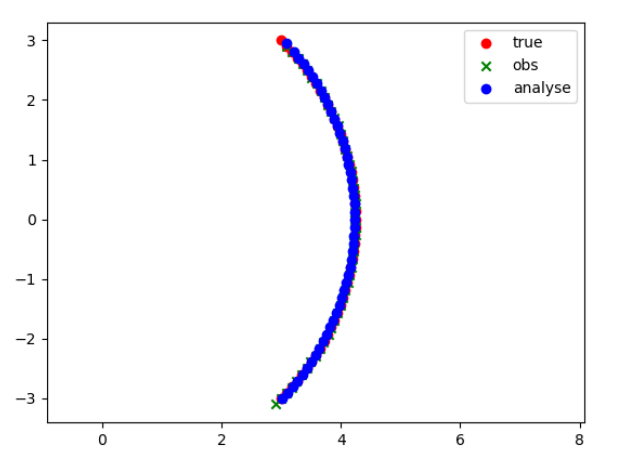
\includegraphics[width=0.45\textwidth]{src/lin2d_pred.png}
    \caption{Prédiction du DAN à l'instant $t=T$ sur les données d'entraînement}
    \label{fig:pred}
\end{figure}

On observe sur la figure \ref{fig:pred} que la trajectoire prédite par le DAN est très proche de la trajectoire réelle : le réseau a bien assimilé les données et a appris à prédire l'état du système. \\

\section{RMSE}

La figure \ref{fig:rmse} montre l'évolution de la RMSE pour les modules (a) et (b) au cours de l'entraînement et de la phase de test. \\

\begin{figure}[H]
    \centering
    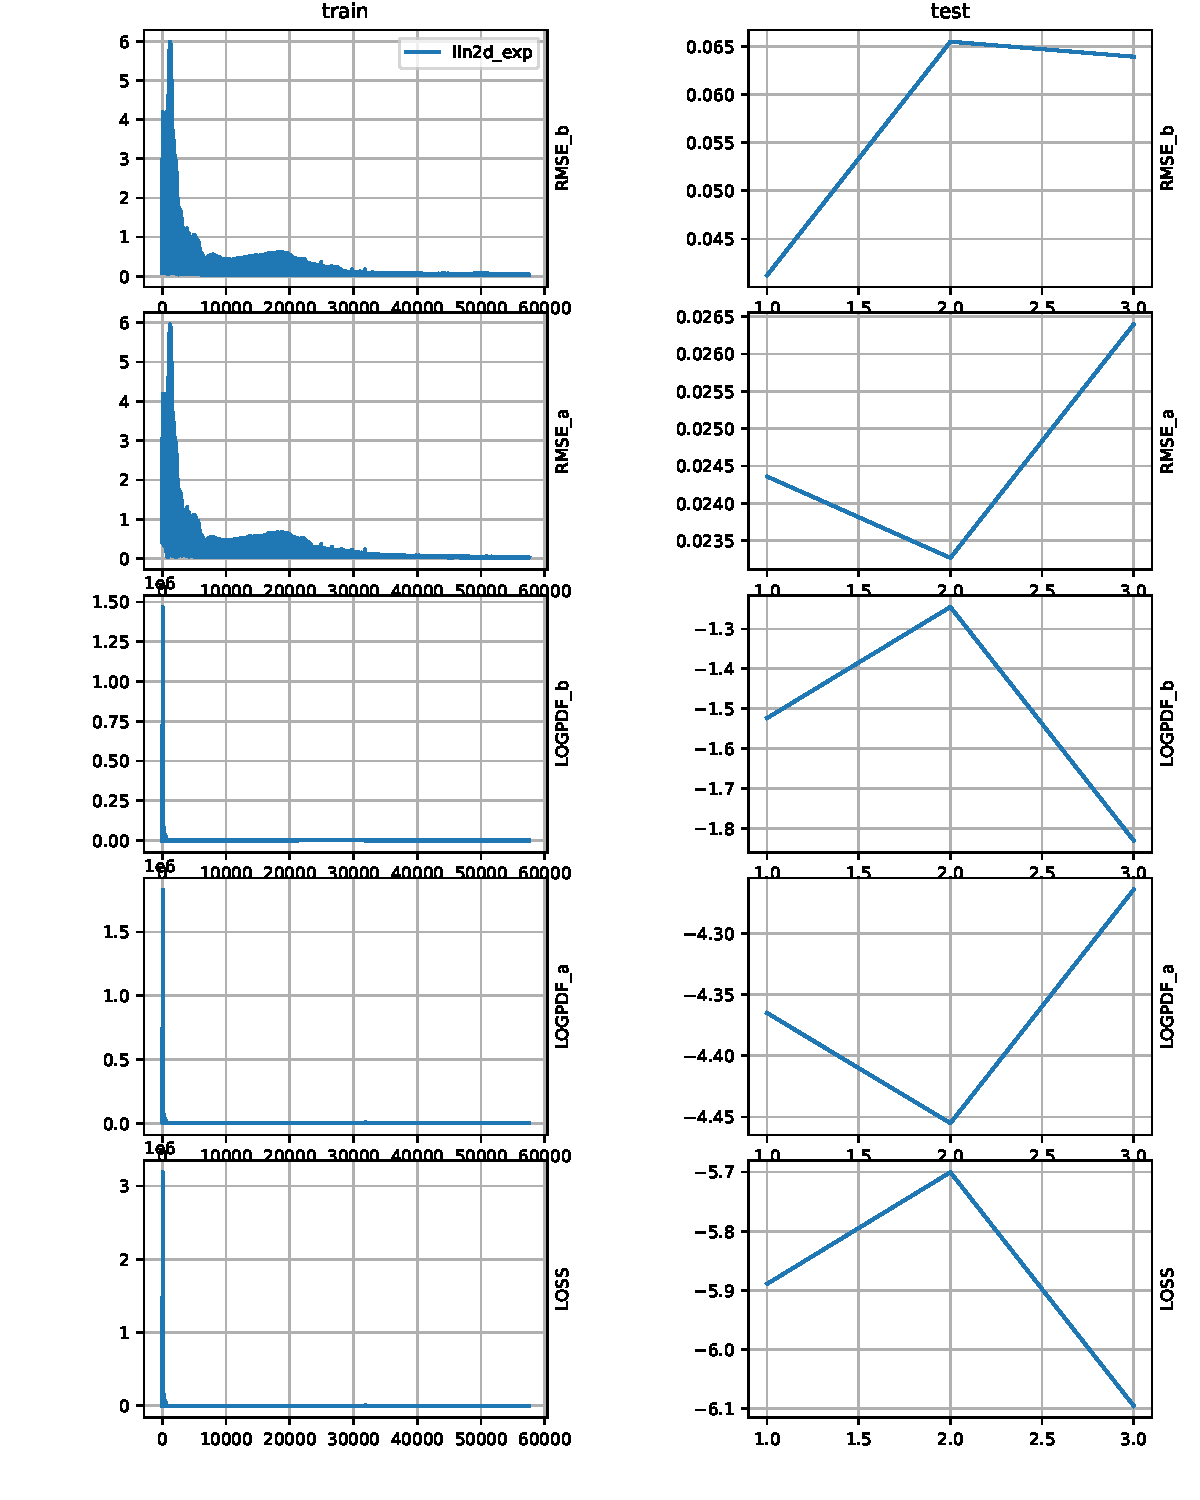
\includegraphics[width=0.85\textwidth]{src/rmse.pdf}
    \caption{Évolution de la RMSE pour les modules (a) et (b) au cours de l'entraînement}
    \label{fig:rmse}
\end{figure}

On observe que la RMSE diminue au fil des itérations pour les deux modules durant l'entraînement, indiquant une amélioration de la performance du DAN. \\
\end{document}